\documentclass[10pt, conference, compsocconf]{IEEEtran}

\usepackage[bookmarks=true]{hyperref}
\usepackage{epsfig}
\usepackage{amsmath,amssymb,amsfonts,latexsym}
\usepackage{enumerate}
\usepackage{xspace}
\usepackage{epsf,picinpar}
\usepackage{varioref}
\usepackage{colortbl,multirow,hhline}
\usepackage{listings}
\usepackage{amssymb}
\usepackage{colortbl,multirow,hhline}
\usepackage{algorithmic}
\usepackage{algorithm}
\usepackage{caption}
\usepackage[normalem]{ulem}
\usepackage{xcolor}
\usepackage{pifont}
\usepackage{xcolor,colortbl}
\usepackage{url}
\usepackage{balance}
\usepackage{graphicx, subfigure}
\usepackage{longtable}
\usepackage{lscape}
\usepackage{multirow}
\usepackage{listings}
\usepackage{framed}
\usepackage{morefloats}
\usepackage[T1]{fontenc}
\usepackage{array}
\usepackage{pdfpages}
\usepackage{fancybox}
\usepackage{amsmath}
\usepackage{flushend}
\usepackage{booktabs}
\usepackage{enumitem}
\usepackage{adjustbox}
\usepackage[charter]{mathdesign}
\usepackage{eulervm}

\renewcommand{\ttdefault}{cmr}

\newcommand{\limit}[1]{\textcolor{red}{\ding{46}~Page limit:~#1}\\}
\newcommand{\todo}[1]{\textcolor{blue}{\ding{46}~#1}} 
\newcommand{\ie}{\emph{i.e.,}\xspace}
\newcommand{\eg}{\emph{e.g.,}\xspace}
\newcommand{\etc}{etc.\xspace}
\newcommand{\etal}{\emph{et~al.}\xspace} 
    
\begin{document}

\title{
	{A Systematic Literature Review on Energy Efficiency in Robotics Software}
}

\author{
\IEEEauthorblockN{dr. Ivano Malavolta}
\IEEEauthorblockA{	
	Supervisor \\ 
	Vrije Universiteit Amsterdam
}

\vspace{5mm}

\IEEEauthorblockN{Stan Swanborn}
\IEEEauthorblockA{S2627602\\
s.o.swanborn@student.vu.nl}
}


\maketitle

\begin{abstract}
\noindent \textit{Context}. 
Nowadays, mobile robots are widely used in many applications. Non-mobile robots are widely used in industrial automation.
This literature study covers the field of research into the energy efficiency of robotics software.

\noindent \textit{Goal}. 
The goal of this literature study is to present a survey of existing research on energy efficiency in robotics software.

\noindent \textit{Method}. 
The method used is a rigorously designed literature study, spanning 17 primary studies. 
These primary studies are summarized, categorized, and analyzed in order to derive relevant patterns across the different studies.

\noindent \textit{Results}. 
The result is given in three parts, as answers to the three research questions. 
The results show that the field of study, while existing since before the change of the century, can still be considered immature.
With attained interest over the last 5 to 10 years.
The results also gave rise to the motivation for the expansion of research into the energy impact of the robotics software itself.
This field of study is still very much in its infancy but proves essential in maximizing energy efficiency of robotic systems, 
as software is the main enabler of robotics, its energy consumption will directly influence the energy consumption of the entire system.

\noindent \textit{Conclusions}.
After reading this literature study, the reader will have gained insight in the state-of-the-art of analyzing and 
improving energy efficiency in robotics software. The reader will be able to judge the findings because of the analyzed publication trends
and will be able to judge if the findings are of use for their personal application using the trade-off analysis.
\end{abstract}

\begin{IEEEkeywords}
Green Software, Robotics Software, Mobile Robots, Energy Efficiency, Systematic Literature Review, Systematic Literature Study
\end{IEEEkeywords}

\section{Introduction}
\label{sec:intro}

% quote from paper 16
% Explains mobile robots and their complications with energy consumption
Mobile robots are widely used in many applications \cite{mei2005energy_consumers_identified}.
People can buy intelligent robotic vacuum cleaners or lawn mowers from stores. 
Some hospitals are using robots to provide quick and safe medicine delivery \cite{evans1994courier_hospital}.

Batteries are often used to provide power for mobile robots; however, they are heavy to carry and have limited energy capacity. 
A Honda humanoid robot can walk for only 30 minutes with a battery pack they carry on the back \cite{aylett2002machines_to_life}; 
energy is the most important challenge for mobile robots. 
Rybski et al. \cite{rybsky2000robot_rangers} show that power consumption is one of the major issues in their robot design.

% Explain Industry4.0 and the impact on energy consumption and society
Robots can also be non-mobile, these robots mostly exist in an industrial setting and form the basis of the fourth industrial revolution,
also called \textit{Industry 4.0} \cite{lasi2014industry4}. 
% Prime examples of multi-robot, Industry 4.0 applications include: material handling \cite{wan2017iot_material_handling}, assembly line \cite{stenmark2015assemblyline_robots}, warehouse maintenance, cooperative navigation \cite{muhlbacher2017multi_robot_navigation} etc.
Industrial firms contribute to 36\% of total global energy consumption and 24\% of total CO2 emissions \cite{international2006energy}.
% Nowadays, the society is putting a growing effort towards reducing greenhouse gas emissions and to reach an environmentally 
% sustainable future. This awareness has brought energy consumption and CO2 emission related objectives to the attention of operations managers in manufacturing companies. 
% In production scheduling decisions, besides time related objectives, energy consumption related objectives have become important \cite{gurel2019industrial_robot_scheduling}. 
Energy consumption in the manufacturing sector has been declining since 1998. 
For instance, in the U.S., the energy consumption in the manufacturing sector decreased by 17\% from 2002 to 2010 \cite{US2018energy_administration}.
Despite these improvements, 
Fysikopoulos et al. \cite{fysikopoulos2012automotive_energy_consumption} assert that 20\% to 40\% unnecessary use of energy may still be found in industrial firms. 
Hence the energy performance of manufacturing systems is a \textit{major area of research} and a concern for many manufacturing companies.

According to the IFR Statistical Department \cite{IFR2010executive_summary}, 
the level of automation in the automobile frame- and body construction process was 90\%, which implies a heavy use of industrial robots in related tasks. 
Also, Engelmann \cite{engelmann2009energy_efficient_factories} states that about 8\% of the total energy consumption in automotive industries belongs to industrial robots. \\

% Explain motivation and goal for this paper and what is explained in what section
Considering the aforementioned, it is logical to understand that the effort to maximize energy efficiency in robotics will have a 
significant impact on the world energy consumption and consequently CO2 emissions.
The \textbf{goal} of this study is to present a survey of existing research on energy efficiency in robotics software.
Industry 4.0, is characterized as a digital revolution.
It is blurring the lines between physical, digital, and biological spheres\footnote{\url{https://www.therobotreport.com/robots-software-software-eating-world/}}.
This complicated this literature study, as will be apparent in section \ref{sec:results}, 
and forms the basis for the motivation for expansion of research into the energy impact of robotics software itself 
- as explained in section \ref{sec:discussion}.

For this study a total set of \textbf{683} potentially relevant studies were identified. 
After the application of the selection procedure, as described in section \ref{sec:study_design:search_selection}, 
the set of \textit{primary studies} consisted of \textbf{17} studies.
\section{Study design}
\label{sec:study_design}
This literature study has been designed and carried out by following 
well-accepted methodological guidelines on secondary studies
\cite{petersen2015guidelines_systematic, kitchenham2013systematic_review_guidelines, wohlin2012experimentation}.

This literature study targets multiple research questions. 
These questions will be given and motivated in subsection \ref{sec:study_design:research_questions}.
Then the search and selection of papers adhering to the inclusion and exclusion criteria began.
This process, and the criteria, are given in subsection \ref{sec:study_design:search_selection}.
After the selection was made final, hereon after called the \textit{primary studies}, the summarization and categorization process began. 
This process is the most important step for writing the literature study; the studies are made comparable by finding the commonalities and patterns in the field of study. 
This process is further explained in subsection \ref{sec:study_design:summ_categor}.


\subsection{Research Questions}
\label{sec:study_design:research_questions}
This study considers three research questions. These questions and their motivations are given in this subsection.

\vspace{5mm}

\textbf{[RQ1]} \textit{What are the publication trends of papers on energy efficiency in robotics software?}

\vspace{5mm}

To be able to judge any characteristics of the state-of-the-art of energy efficiency in robotics software, one needs to know the maturity of the field.
What publication trends are observed?

\vspace{5mm}

\textbf{[RQ2]} \textit{What is the state-of-the-art on analyzing and improving the energy efficiency in robotics software?}

\vspace{5mm}

This research question aims to answer what the state-of-the-art is for achieving and analyzing an increase of energy efficiency in robotics software.

\vspace{5mm}

\textbf{[RQ3]} \textit{What are the trade-offs when dealing with energy efficiency in robotics software?}

\vspace{5mm}

This research question aims to give insights into what Quality Attributes have been identified to trade-off with energy efficiency. 
It is valuable for researchers and practitioners to know that if one wants to increase energy efficiency, one can expect a decrease of some other attribute.

\subsection{Search and Selection}
\label{sec:study_design:search_selection}
\begin{figure}
    \centering
    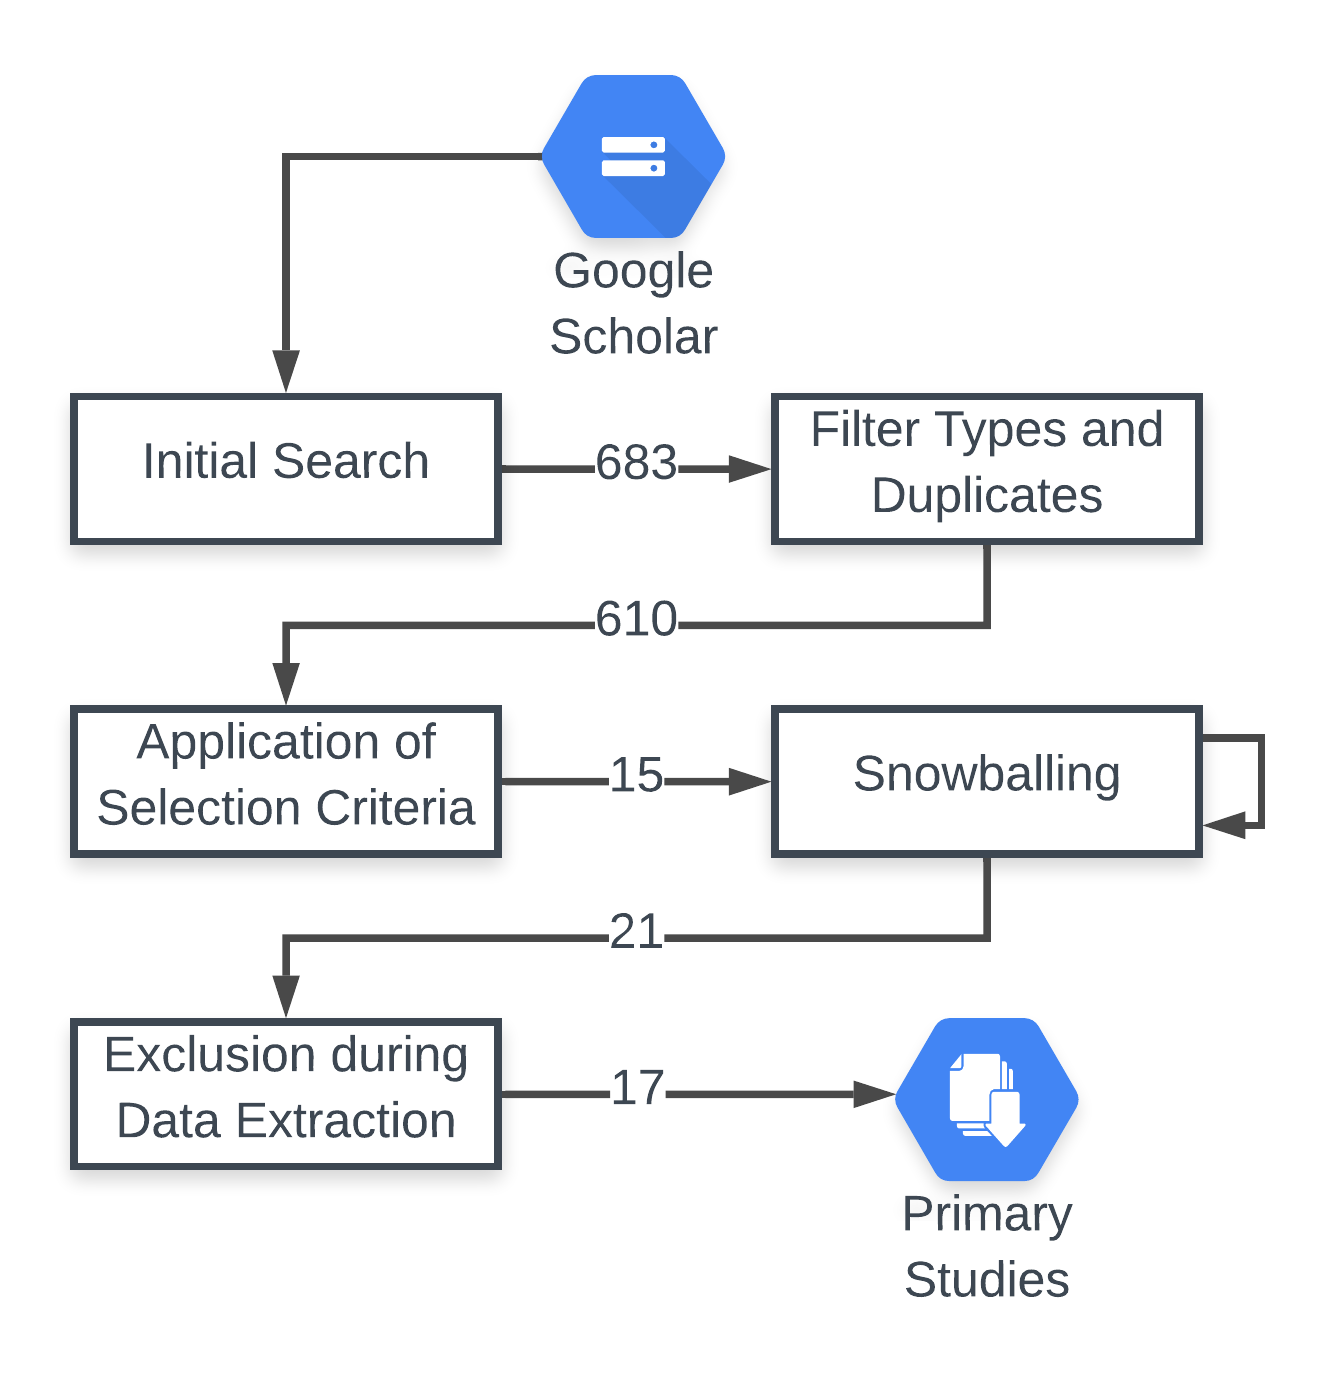
\includegraphics[width=0.5\textwidth]{figures/selection_process_var2.png}
    \caption{The Search and Selection process}
    \label{fig:search_selec_process}
\end{figure}

The \textit{study design} is agreed and approved upon before starting the search and selection process. 
This is meant to prevent, as much as possible, any personal bias during search and selection, as the \textit{search string} and \textit{selection criteria} are already finalized.
This, and more threats to the validity of this report are detailed in section \ref{sec:threats}.
An overview of the search and selection process is given in figure \ref{fig:search_selec_process}.
The process, as displayed in the figure, is further elaborated on in this subsection.

\vspace{5mm}

\noindent\textbf{1. Initial Search:}
For the initial search, \textbf{Google Scholar}\footnote{\url{https://scholar.google.com/}} was used. 
Google Scholar is at the time of writing one of the largest and most complete database and indexing system for scientific literature.
It has been used as a data source for the following main reasons:
\begin{enumerate}
    \item The adoption of this indexer has proved to be a sound choice to identify the initial set 
    of literature studies for the snowballing process \cite{wohlin2014snowballing}.
    \item The query results can be automatically extracted from the indexer using Zotero\footnote{\url{https://www.zotero.org/}}.
\end{enumerate}

\begin{figure}
    \centering
    \textit{"(intitle:robot) AND (intitle:power OR intitle:green OR intitle:energy OR intitle:battery) AND software"}
    \caption{Search String}
    \label{fig:search_string}
\end{figure}

The results were retrieved using the \textbf{search string} as given in figure \ref{fig:search_string}. 
The search string is kept as general as possible so that potentially relevant studies that would be able to make it 
to the primary studies but might not match exactly, are not accidentally filtered out by the automatic search.

The search string consists of three main components, each is given and motivated below:
\begin{enumerate}
    \item \textit{intitle: robot} \newline
    Considering this literature study explicitly focuses on \textbf{robotics}; 
    the inclusion of \textit{robot} is warranted in the search string to retrieve studies in the context of robotics.

    \item \textit{intitle: power \textbf{OR} green \textbf{OR} energy} \newline 
    Considering this literature study explicitly focuses on \textbf{energy efficiency};
    the inclusion of \textit{power} \textbf{OR} \textit{green} \textbf{OR} \textit{energy} related titles is warranted in the search string to retrieve studies focussing on 
    these concepts.
    These concepts are deliberately logically seperated with an \textbf{OR} operator to prevent the exclusion of any studies that only focus on a subset.

    \item \textit{software} \newline
    Considering this literature study explicitly focuses on \textbf{software};
    the inclusion of software related papers is warranted.
    This is the only concept that is not explicitly limited to the \textbf{title}, as it is a broad, general term which might not always be mentioned
    explicitly in the title but does get mentioned in the abstract or keywords.
    
\end{enumerate}
The number of results at the time of performing the initial search were \textbf{683} potentially relevant studies.

\noindent\textbf{2. Filter Types and Duplicates}
During this step, all publication types that are not peer-reviewed by nature are filtered out. 
The potentially relevant studies that resulted from the initial search were thus automatically filtered to be only of any of these types: 
\textit{Journal Articles, Conference Papers, Book Sections}.
By filtering these types, the total number of potentially relevant studies went down to \textbf{615}. 
Then, the filtered collection was filtered automatically once more on 
syntactic (i.e. papers which are exactly the same) duplicates. 
Semantic (i.e. different papers about the same approach) duplicates were left to be filtered out manually during the data extraction phase, as explained in
\ref{sec:study_design:summ_categor}, in order to prevent unintentional removal. 
However, the approach as followed by this literature study is given for both below:

\vspace{1mm}

\begin{enumerate}
    \item[\textit{Syntactic}] In the case of a syntactic duplicate, only one record was kept. 
    These duplicates are in essence exactly the same, therefore which record to keep is not relevant.
    However, if applicable, the latest version (latest publication year) has been kept.

    \item[\textit{Semantic}] In the case of a semantic duplicate, meaning a paper was published in more than one instance 
    (for example, if a conference paper was extended to a journal version), only one instance has been counted as a primary study. 
    In those cases the journal version of the study has been preferred, as it is supposed to be the most complete; nevertheless, 
    both versions have been used in the data extraction phase and in the analysis of the publication trends (RQ1, see section \ref{sec:results}).

\end{enumerate}
After the duplicates were removed the total number of potentially relevant studies decreased to \textbf{610}.

\vspace{5mm}

\noindent\textbf{3. Application of Selection Criteria:}
During this step the \textbf{610} potentially relevant studies are filtered by applying the selection criteria. 
The study is added to the set of \textit{primary studies} in case it satisfies \textbf{all} of the inclusion criteria (\textit{i1-i5}) and \textbf{none} of the exclusion criteria (\textit{e1-e5}). 
These criteria consist of:
\begin{itemize}
    \item[i1] Studies focussing on robotics.
	\item[i2] Studies focussing on energy efficiency.
    \item[i3] Studies focussing on software aspects.
    \item[i4] Studies providing evaluation.
    \item[i5] Studies that are peer-reviewed.
    \item[i6] Studies written in English.
    
	\item[e1] Studies that, while focussing on energy efficiency, do not explicitly deal with any software aspect.
    \item[e2] Studies where energy efficiency is only used as an example.
    \item[e3] Secondary or Tertiary studies (literature reviews, theses etc).
    \item[e4] Studies that are not in the form of a Journal Article, Conference Paper, Book or Book Section.
    \item[e5] Studies not available as full-text.
\end{itemize}

The application of the selection criteria was done manually by following the steps given below. 
Each step was performed to see if any selection criteria could be decided based on the information gained by it. 
If a step decided one of the \textit{exclusion criteria} the next steps were not followed for that particular study, 
as it already warrants rejection. 
The following steps were followed for each of the \textbf{610} potentially relevant studies:
\begin{itemize}
	\item[S1] Read the \textit{Title}.
	\item[S2] \textit{Download} the study.
	\item[S3] Read the \textit{abstract}.
	\item[S4] Read the study \textit{full-text}.
\end{itemize}

Once the application of the selection criteria was completed for the entire set of potentially relevant studies,
a total of \textbf{15} papers were identified to satisfy \textbf{all} of the \textit{inclusion criteria} and
\textbf{none} of the \textit{exclusion criteria}. These formed the set of \textbf{considered studies}.

\vspace{5mm}

\noindent\textbf{4. Snowballing:}
% This table is not for snowballing, but does not want to move a page up if not put here.
% Even while using the [t] option.
\begin{table*}[t]
    \centering
    \caption{Data sheet columns.}
    \begin{tabular}{cllc}
        \toprule
            ID &
            Column Name & 
            Example Value & 
            Relevant RQ  \\
        \midrule
            1 &
               Date & 
                \textit{2020} & 
                RQ1 \\

            2 &
                Energy Metric & 
                \textit{FPS / W (Watt)} & 
                RQ2 \\

            3 &
                QA Trade-off & 
                \textit{Performance vs Efficiency} & 
                RQ3 \\
                
            4 &
                Application Domain & 
                \textit{Robot Exploration} & 
                RQ2 \\

            5 & 
                Identified Major Consumers & 
                \textit{Too many stops and turns in path} & 
                RQ2 \\

            6 & 
                Identified Improving Software Aspect & 
                \textit{Improved path finder} & 
                RQ2 \\
            
            7 &
                Major Contribution & 
                \textit{The actual improved, evaluated, path finder algorithm} & 
                RQ2 \\
            
            8 &
                Experiment & 
                \textit{None / Simulation / Real-World / Combination} & 
                RQ2 \\
            
            9 &
                Comparison Against State-Of-The-Art & 
                \textit{Yes / No} & 
                RQ2 \\
            
            10 &
                Energy Model &
                \textit{1 Unit of Distance = 1 Unit of Energy} & 
                RQ2 \\
        \bottomrule
    \end{tabular}
    \label{table:data_sheet}
\end{table*}
In this phase the automatic search was complemented with recursive \textit{backward} and \textit{forward} snowballing \cite{wohlin2014snowballing}.
During the \textit{backward} snowballing, all references of each \textit{considered study} were added to the potentially relevant studies. 
After each reference from each considered study was added, the steps for applying the selection criteria, as given above, were once more followed. 
After completing this iteration, each newly considered study was also used in the recursive backward snowballing process.

Following the backward snowballing, \textit{forward} snowballing was used. 
In this process each study that cites each considered study is added to the potentially relevant studies, hereafter each step for applying the selection criteria was once more followed, and the newly considered studies were recursively used in the forward snowballing process.

\vspace{5mm}

On completion of the snowballing process, the set of considered studies grew to \textbf{21} studies. These studies now form the \textit{primary studies} set.

\vspace{5mm}

\noindent\textbf{5. Exclusion during Data Extraction:}
Papers that made it to the collection of primary studies can still be removed from the set during the data extraction phase if they 
are found to satisfy one of the \textit{exclusion criteria} while reading the study full-text.

What the data extraction phase consists of, is explained in section \ref{sec:study_design:data_extract}.

For this literature study, a total of \textbf{4} papers have been excluded during data extraction. 

\subsection{Data Extraction}
\label{sec:study_design:data_extract}
During the data extraction phase, each \textit{primary study} is read full-text and its findings are used to construct a data sheet.
This data sheet aims to cover all similarities and patterns between the primary studies so that this literature study can be written, comparing their findings.
The data sheet was improved in multiple iterations, discussing each iteration with my supervisor.

The data sheet constructed during this phase; its columns, example values and their most relevant RQ are given in table \ref{table:data_sheet}.

\subsection{Data Synthesis}
\label{sec:study_design:data_synth}
Arriving at this step, the set of \textit{primary studies} is finalized, now consisting of \textbf{17} papers.
During the data synthesis phase, the filled out datasheet, as given in appendix \ref{appendix:data_sheet_1} and \ref{appendix:data_sheet_2}, 
was used to plot the results and gain insights.
These are given in section \ref{sec:results}.
\section{Results}
\label{sec:results}
As stated in the introduction, section \ref{sec:intro}, this literature study was complicated by 
the blurring lines between physical, digital, and biological spheres.
This literature study set out to discover the state-of-the-art of research on the energy efficiency impact of, \textbf{explicitly} \textit{robotics software}.
Meaning the explicit impact on energy efficiency of various aspects of the software itself.
It became quickly apparent during the search and selection process, as described in section \ref{sec:study_design:search_selection}, 
that few studies existed on this specific topic.
Out of all 683 potentially relevant studies, only two studies have been found that explicitly research this topic.

\vspace{2mm}

One study \cite{rahman2019cloud_robot_offloading} provides proof that a software architectural change; 
from on-board calculations to off-loading to more available robots or the cloud, actually impacts energy efficiency positively.
Another study \cite{hou2017novel_cloud_evaluation_model} presents a robotics software evaluation method based on energy consumption.
The method allows for identifying those robotics software aspects that consume relatively more energy. 
It can also be used to predict the energy consumption of a specific piece of robotics software, allowing it to be used during software development, 
to create more energy efficient software from the moment it is designed.

\vspace{2mm}

The fact that these two studies were the only ones explicitly covering research into the energy efficiency impact of robotics software aspects will
form the basis of the discussion, given in section \ref{sec:discussion}.
To prevent an insignificant literature study, the focus has been shifted from looking at software aspects, to see what impact 
robotics software in general can have on energy efficiency. The blurred distinction between software and hardware in robotics made the 
application of the inclusion criteria a tough process.
The final selection of primary studies is the result of a rigorous application of these criteria; 
a study had to explicitly cover \textit{some} software aspect in relation to energy efficiency.

\vspace{2mm}

In this section, the insights gained from the data sheet are summarized and given for each column in subsection \ref{sec:results:insights}.
Hereafter, this section is structured according to the research questions.
Each of those subsections gives a detailed explanation of the findings of this literature study in the context of that research question.
The main findings of each research question are presented at the end of each corresponding subsection.

% ========================================================================= Insights =========================================================================

\subsection{Data sheet insights}
\label{sec:results:insights}
The insights, as gained by each of the columns of the data sheet, are given in this subsection.
Any conclusions drawn from these insights in order to answer the research questions targeted by this literature study,
are given in their respective subsections \ref{sec:results:rq1_pub_trends}, \ref{sec:results:rq2_state_of_the_art} and \ref{sec:results:rq3_trade_off}.

\vspace{5mm}

\noindent\textbf{1. Date:}
In figure \ref{fig:pub_trends}, it can be observed that, even though this field of study has been around since before the change of the century,
it truly attained interest in the last decade (2010 - 2020), with a significant spike nearing 2020.
It can also be observed that the more thoroughly peer reviewed, higher quality research; journal articles are only published in the last $\pm 5$ years.

\begin{figure}[t]
    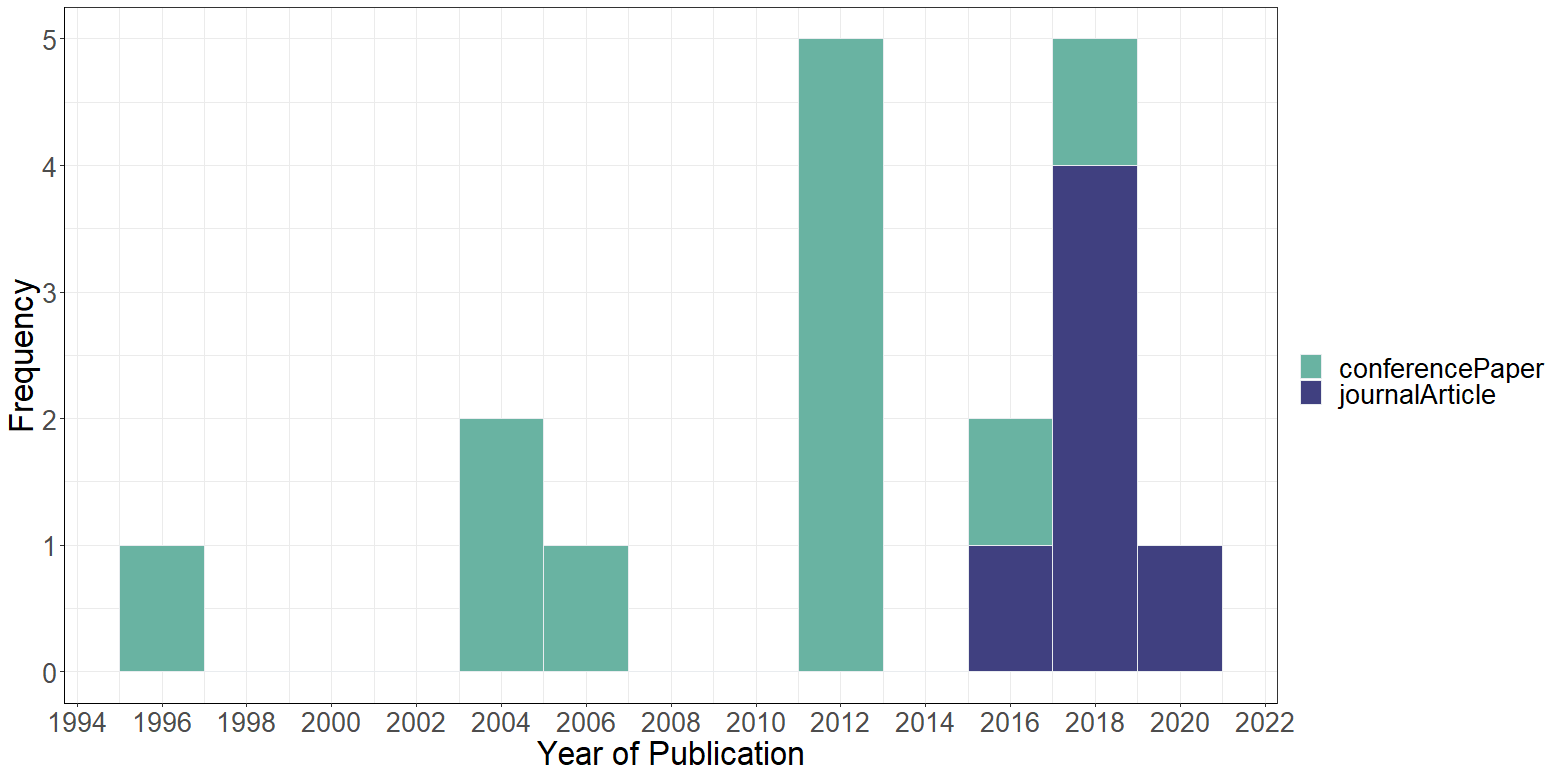
\includegraphics[width=250pt]{figures/publication_trend_extended.png}
    \caption{Publication trends by type}
    \label{fig:pub_trends}
\end{figure}

\vspace{2mm}

\noindent\textbf{2. Energy Metric:} % Might be more sensible to change to Efficiency Metric
% Various metrics used
% Power and Energy separate
% Joules / KiloJoules / NanoJoules most popular.
% Most intersting: FPS / W etc.
% Conclusion: Many different metrics, joules most popular, comparison difficult
It can be observed that the energy metric used in the primary studies differs significantly.
In the case that a simplified energy model is used, as explained in part 10 of this subsection, the energy metric is the most unique;
units of distance traveled per units of energy \cite{mei2006mobile_exploration, patel2012exploration_strategy}.

All other energy metrics given use a study specific metric in relation to either; energy, \textbf{Joules} (\textit{J}) or power, \textbf{Watts} (\textit{W}).
The three most common, descriptive and comparable metrics observed are:
\begin{enumerate}
    \item $FPS / Watt$ \cite{cheng2018FPGA_image_recognition}
    \item $Joules / Meter$ \cite{licea2013wireless_comms}
    \item $Joules / H$ or $Watts / H$ \cite{kim2016firefighting_robot,barili1995efficient_motion}
\end{enumerate}

\vspace{2mm}

\noindent\textbf{3. QA Trade-off:}
% Various trade-offs mentioned.
% Used in RQ 3.
\todo{Write after RQ3}

\vspace{2mm}

\noindent\textbf{4. Application Domain:}
% Exploration / Service robots
\begin{figure}[t]
    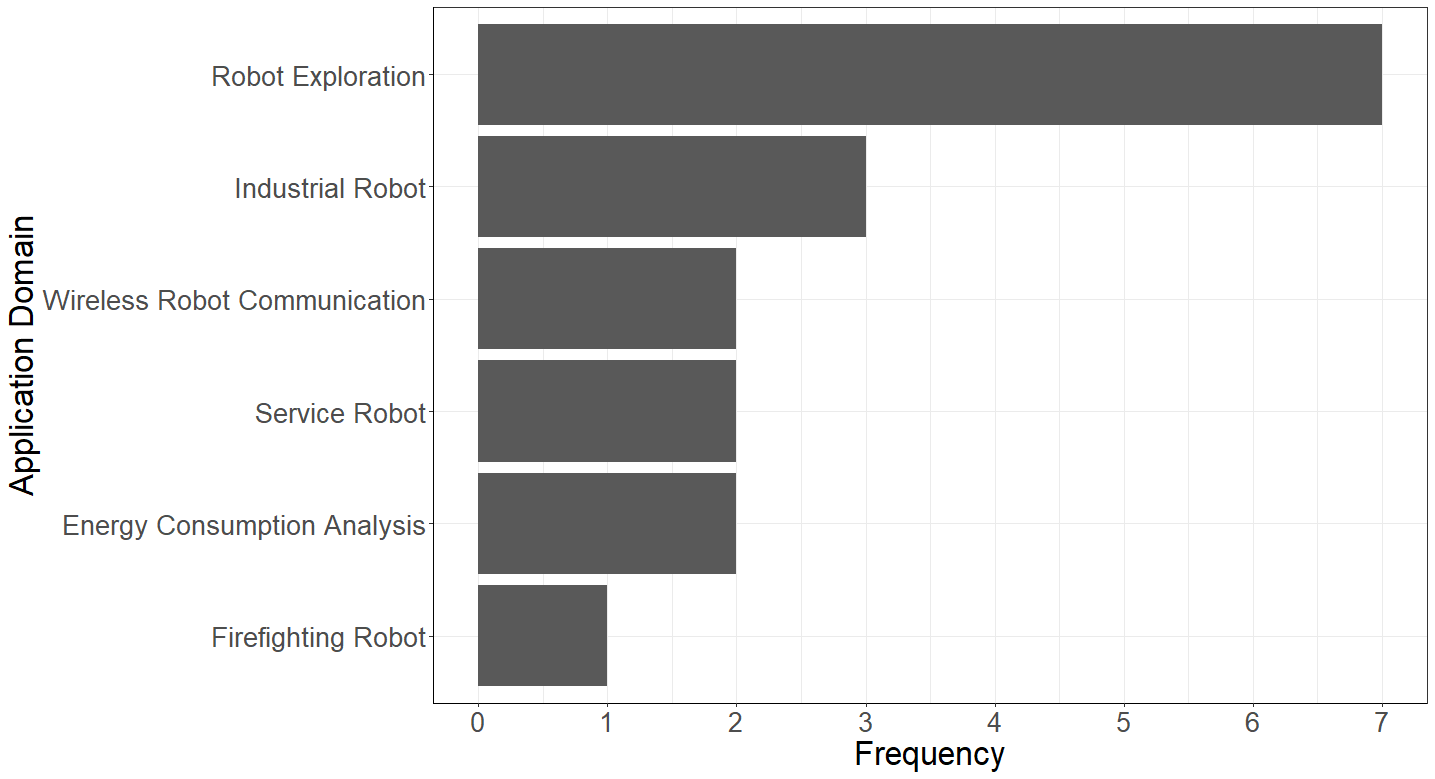
\includegraphics[width=250pt]{figures/app_domains_freq.png}
    \caption{Application domains frequency}
    \label{fig:app_domains}
\end{figure}
In figure \ref{fig:app_domains} it can be observed that the application domain of \textbf{Robot Exploration} is the most frequent
domain considered in the primary studies. 
The domain of \textbf{Industrial Robot} is at the second place with less than half the frequency.

This is interesting, considering that in terms of emmissions and energy saving potential, there is far more to achieve in the industrial domain
as specified in the introduction; section \ref{sec:intro}.
From this statistic one could thus reason that the combination of functional and efficiency improvements forms the main motivation. 
The extension of the operational time of a mobile robot, as a result of the improved energy efficiency, 
is far more functionally relevant than reducing the energy consumption of an industrial robot;
considering the industrial robot has a continuous power supply, energy efficiency is not as functionally important as it will
not deliver any functional improvement. 
Rather, as specified in part 3 (QA Trade-off) of this subsection, it will most likely have some (negative) impact on performace.

\vspace{2mm}

\noindent\textbf{5. Identified Major Consumers:}
% Software inefficiencies
% Hardware inefficiencies
% Hardly win-win, only when time reduced, hardware inefficiency reduced etc. (only with software?)
The identified major consumers in the primary studies vary considerably, as can be seen in appendix \ref{appendix:data_sheet_1}.
This is a result from the different application domains and their implementation specific details.
However, a common theme can be identified:

\vspace{2mm}

No matter the application domain, any identified inefficiency is always traced back to a hardware inefficiency, 
which is solved by improving software.

\vspace{2mm}

Considering robots use software to control their physical hardware, and the fact that robots exist to satisfy some physical need, this makes sense.
From all primary studies, only one identifies solely software itself as the main consumer \cite{hou2017novel_cloud_evaluation_model}.
It presents a novel cloud evaluation model; which evaluates the energy efficiency of the software itself.
Using the model, the software itself; its execution, can be made more efficient.

\vspace{2mm}

The fact that this is the only study addressing this aspect of robotics software, forms the basis of the discussion in section \ref{sec:discussion}.


\vspace{2mm}

\noindent\textbf{6. Identified Improving Software Aspect:}
% Mostly solving hardware with software
Among the primary studies, all inefficiencies are solved by improving the robotics software;
as this literature study explicitly targets such studies.
As the presented improvements are very implementation specific, they are hardly comparable.
However, a common theme among the improvements can be identified:
Each improvement solves a hardware inefficiency using software; however, each improvement does so to various degree.
Two examples from the primary studies:

\begin{itemize}
    \item Improving the path planning algorithm (\textit{software}) to limit inefficient use of \textit{hardware} as the path
    is more energy efficient (shorter, less stops and/or turns, etc.) (\textbf{low degree of improved hardware ineffiency}) \cite{mei2006mobile_exploration}.
    \item Introducing an algorithm (\textit{software}) which off-loads computations to a more energy-optimized cloud infrastructure (\textit{hardware}) 
    (\textbf{high degree of improved hardware inefficiency}) \cite{rahman2019cloud_robot_offloading}.
\end{itemize}

\vspace{2mm}

\noindent\textbf{7. Major Contribution:}
% For example the entire system, integrating the software aspects to improve inefficiency.
For each of the primary studies the major contribution is the implementation and evaluation of the identified software aspect that would
improve the inefficiency. 
This column can therefore be seen as an extension of the previous column (\textit{6. Identified Improving Software Aspect}).

\vspace{2mm}

\noindent\textbf{8. Experiment:}
% Experiment performed most common: simulation, why?
\begin{figure}
    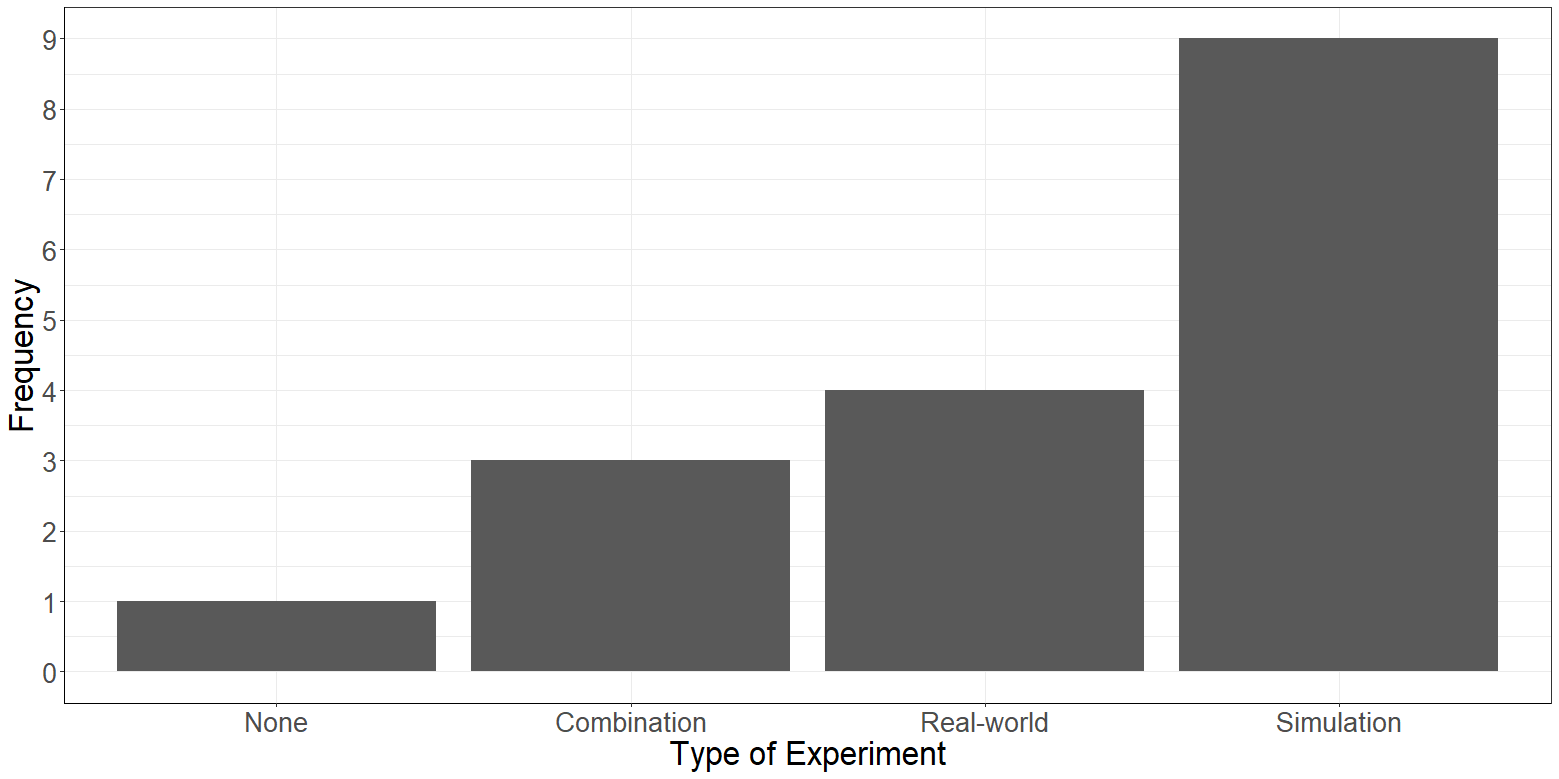
\includegraphics[width=250pt]{figures/experiment_distr.png}
    \caption{Experiment distribution}
    \label{fig:experiment_distr}
\end{figure}
Most studies performed an experiment, only one primary study did not.
From figure \ref{fig:experiment_distr}, it can be observed that most studies (9) perform an experiment in the form of a simulation, 
this is without counting the combination of real-world and simulation.
considering those would bump the number of primary studies using a simulation as experiment to 12, $\pm 70\%$ of the primary studies.
Four primary studies performed a real-world experiment.
Three studies performed a combination of real-world and simulated experiments.

For understanding the experiments, especially the simulations, the energy model used is of high value; this is given in appendix \ref{appendix:data_sheet_2}.

\vspace{2mm}

\noindent\textbf{9. Comparison Against State-Of-The-Art:}
% Mostly yes, important for validity!
To verify the validity of the claims presented in the primary studies, the comparison against the state-of-the-art is important.
In 14 of the 17 primary studies ($\pm 80\%$) a comparison was made.
From the three studies that had no comparison, one was a paper presenting a novel cloud evaluation model \cite{hou2017novel_cloud_evaluation_model}
which has no state-of-the-art to compare to as it presents something completely new.

\vspace{2mm}

It is therefore safe to say that 15 of the 17 primary studies ($\pm 90\%$) uphold the comparison.

\vspace{2mm}

This is of importance as this literature study's validity is dependent upon the validity of the literature it is based on.
The threats to the validity of this literature study, and what has been done to mitigate these threats,
is further detailed in section \ref{sec:threats}.

\vspace{2mm}

\noindent\textbf{10. Energy Model:}
% Interesting for future research / comparison between the relative studies
The energy model used in any of the primary studies is given in appendix \ref{appendix:data_sheet_2}.
The validity of the contributions of the studies is dependent on the validity of the energy model used (if applicable), 
therefore these are recorded and given.

\vspace{2mm}

They can also be valuable for any practitioner or researcher that seeks insight into energy models for simulation.

\vspace{2mm}

Many different energy models have been used by the various primary studies, some try to simulate the energy consumption 
as precisely as possible by simulating drag, torque, acceleration, decelleration, etc. with advanced mathematics. 
Two papers \cite{patel2012exploration_strategy, mei2006mobile_exploration}, use the same approach as their energy model.
The energy model used is very simple and it is the only model in the primary studies which is used by multiple papers;
these papers are written by different authors but within the same field of study; mobile robot exploration.
The model they use consists of a simulated grid, where each grid cell consists of 1x1 Units of Distance, 
and travelling 1 Unit of Distance equals 1 Unit of Energy.
Each stop costs 0.5 Units of Energy and each 45° turn costs 0.4 Units of Energy, each additional 45° adding another 
0.2 Units of Energy to the total cost.
Meaning: a 90° turn would cost 0.6 Units of Energy and a 135° turn would cost 0.8 Units of Energy etc.

\vspace{2mm}

This simple energy model is only relevant for simulating the energy cost of moving the robot.
It is however interesting, that none of the energy models, not even the mathematically advanced ones, are capable of 
simulating any computational energy usage.
Therefore, in studies where this is of importance, only a real-world experiment was able to provide these insights.

% ========================================================================= RQ 1 =========================================================================

\subsection{Results - publication trends (RQ1)}
\label{sec:results:rq1_pub_trends}

In this section the results obtained when analyzing the publication trends on energy efficiency in robotics software are presented.
Understanding the publication trends in the field of study is essential for interpreting the results of this literature study as it gives
an idea of the maturity of the field.

From these findings, as stated in part 1. of subsection \ref{sec:results:insights}, we can conclude that the maturity of the field, considering the number of publications relative to their publication dates, 
is rather limited the further back we go in time. It is important to take this into account for both the findings of this literature study, presented in the following subsections 
\ref{sec:results:rq2_state_of_the_art} and \ref{sec:results:rq3_trade_off}, and for the discussion as presented in section \ref{sec:discussion}.
Considering the aforementioned difficulty with the initial goal of this literature study; from the publication trends we can see that this 
is probably the case because of a rather immature field of study.

\vspace{5mm}

\noindent\fcolorbox{black}[HTML]{FFFFFF}{\parbox{0.47\textwidth}{%
\noindent \textbf{Main Findings.}
\begin{enumerate}[nolistsep]
\item The field of study has been around since before the change of the century.
\item The field can still be considerd immature as publications only recently attained in numbers.
\end{enumerate}}}

% ========================================================================= RQ 2 =========================================================================

\subsection{Results - state-of-the-art (RQ2)}
\label{sec:results:rq2_state_of_the_art}
In this section the state-of-the-art in analyzing and improving energy efficiency in robotics software is presented as found from studying the primary studies.

\noindent\textbf{1. Analyzing:}
The novel cloud evaluation method \cite{hou2017novel_cloud_evaluation_model}, introduces a whole new paradigm in robotics software.
This can be concluded as it is the only paper out of 683 potentially relevant studies, and 17 primary studies, 
that explicitly looks at the execution of robotics software itself for improvement of energy efficiency.

It presents a novel method to evaluate the energy efficiency of a specific piece of software.
The method can be used on existing software, to identifiy bottlenecks, or used during the development of the software itself;
providing the ability to improve the energy efficiency of the software execution during design time.

It can be considered the state-of-the-art of evaluation and analysis, in robotics software.
However, it should be considered that this was the only paper that focussed so explicitly on software and its impact on energy.
Considering the 16 other primary studies, and the observations made as stated in part 8 of subsection \ref{sec:results:insights}; 
it can be stated that another big standard in this field is the evaluation through practice; 
in the form of a simulation, a real-world experiment or a combination thereof.

\vspace{5mm}

\noindent\textbf{2. Improving:}
The methods to improve energy efficiency in robotics software vary significantly across the primary studies. 
As stated in part 5 and 6 of subsection \ref{sec:results:insights}; a trend observed is that they mostly solve hardware (physical) 
inefficiencies using software solutions, like an improved algorithm.

\vspace{2mm}

As stated before, this literature study initially set out to research the state-of-the-art in terms of improving the
energy efficiency of robotics software \textit{itself}.
The fact that only two of the primary studies presented such research forms the basis of the discussion in section \ref{sec:discussion}, 
this section will therefore detail what has been found by studying the primary studies in the context of improving energy efficiency 
by \textit{using} robotics software.

\vspace{2mm}

Each primary study presented an evaluated software solution that improves energy efficiency.
The prime techniques extracted from the primary studies consist of:

\vspace{2mm}

- The technique to off-load computations to other, nearby, robots that are more 'available' 
(i.e. robots that have more resources available for such computations relative to the current one.), or to off-load it to the cloud.
The concept here is that the cloud infrastructure (hardware itself, hardware utilization, etc) is more energy-optimized compared to the
hardware used on the robots themselves, and will thus result in an improved energy efficiency.
Even though some energy is wasted in the transmission of data, the overall energy consumption is decreased \cite{rahman2019cloud_robot_offloading}.
    
\vspace{2mm}

- The technique to improve the path finding for mobile robot exploration. 
Many existing studies select the next target based on the utilities and costs of the frontier cells 
\cite{burgard2005multi_robot_exploration, simmons2000multi_robot_exploration,zlot2002multi_robot_exploration} 
However, study \cite{mei2006mobile_exploration} proves that if the next target is selected based on the orientation of the robot, 
that overlap in the robot trajectory is guaranteed to be impossible. This decreases inefficiency by nature, and thus improves energy 
efficiency.
    
\vspace{2mm}

- The technique to limit stops, directional changes (turns) and the degree to which the direction is changed as much as possible 
significantly improves energy efficiency. By the very nature of this technique, an improved obstacle detection and avoidance algorithm
is needed for mobile robotic systems. This technique is widespread over the primary studies, and presented and evaluated in 
\cite{xie2018mecanum_wheel, kim2016firefighting_robot, benkrid2016multi_robot_exploration, barili1995efficient_motion, 
jia2004grid_strategy_exploration, mei2005energy_consumers_identified, patel2012exploration_strategy}.
    
\vspace{2mm}

- The technique to limit motion at high speeds, with numerous moments of acceleration and decelleration
\cite{wingstrom2013robot_cell_scheduling}.
    
\vspace{2mm}

- The technique to prevent idle time as much as possible \cite{gurel2019industrial_robot_scheduling, 
kaitwanidvilai2020industrial_robot_cycle_time, wingstrom2013robot_cell_scheduling}.
    
\vspace{2mm}

- The technique to limit data transmission by preventing the transmission of duplicate data in distributed robotic systems \cite{huh2013distributed_swarm}.

\vspace{2mm}

- The technique to limit physical inefficiencies (e.g. loss of traction because of payload weight), if possible, by adding more robots to the system which would cause the overall
energy consumption to go down as the physical inefficiency (now solved) was consuming more energy than the addition of the subrobots \cite{kim2016firefighting_robot}.
    
\vspace{2mm}

- The technique to use more advanced hardware (i.e. more energy-optimized, desktop grade, hardware instead of custom robotic hardware) 
on robots in combination with energy-optimized software to improve energy efficiency significantly \cite{cheng2018FPGA_image_recognition}.
    
\vspace{2mm}

- The technique that sacrificing some energy on finding a better position for the transmission of data over a wireless connection
(a higher channel gain) will ultimately improve energy efficiency as less time is spend and wasted on (re)transmitting 
data over a bad wireless connection \cite{licea2013wireless_comms}.

\vspace{5mm}

\noindent\fcolorbox{black}[HTML]{FFFFFF}{\parbox{0.47\textwidth}{%
\noindent \textbf{Main Findings.}
\begin{enumerate}[nolistsep]
\item The most common way to analyze the energy efficiency of robotics software consists of performing experiments, evaluating the results.
\item The state-of-the-art on improving the energy efficiency consists of:
    \begin{enumerate}
        \item Off-loading computations to more energy-optimized infrastructure.
        \item Improved path finding, obstacle avoidance etc.
        \item Limit physical inefficiencies, idle time, acceleration, decelleration, stops, turns, directional changes and the extent of the directional change.
        \item The use of more energy-optimized hardware on robotics themselves.
        \item Sacrificing some energy to achieve higher efficiency, f.e. finding a better location with better signal for data transmission.
    \end{enumerate}
\end{enumerate}}}

% ========================================================================= RQ 3 =========================================================================

\subsection{Results - energy QA trade-off (RQ3)}
\label{sec:results:rq3_trade_off}
From the primary studies it became quickly apparent that no significant improvement of energy efficiency came without the cost
to some other attribute. These trade-offs have been mapped to 
\textit{system Quality Attributes\cite{iso2011quality_attributes}} and will be presented
in this section.

This section aims to give insight into the various costs that have been associated with improving energy efficiency.
Any reader can judge if any QA trade-off is manageable in the context of their own system, when applying the paradigms
described in subsection \ref{sec:results:rq2_state_of_the_art}. 
The QA's that trade-off with improving energy efficiency are further detailed and related to findings from the primary studies below.

\begin{figure}
    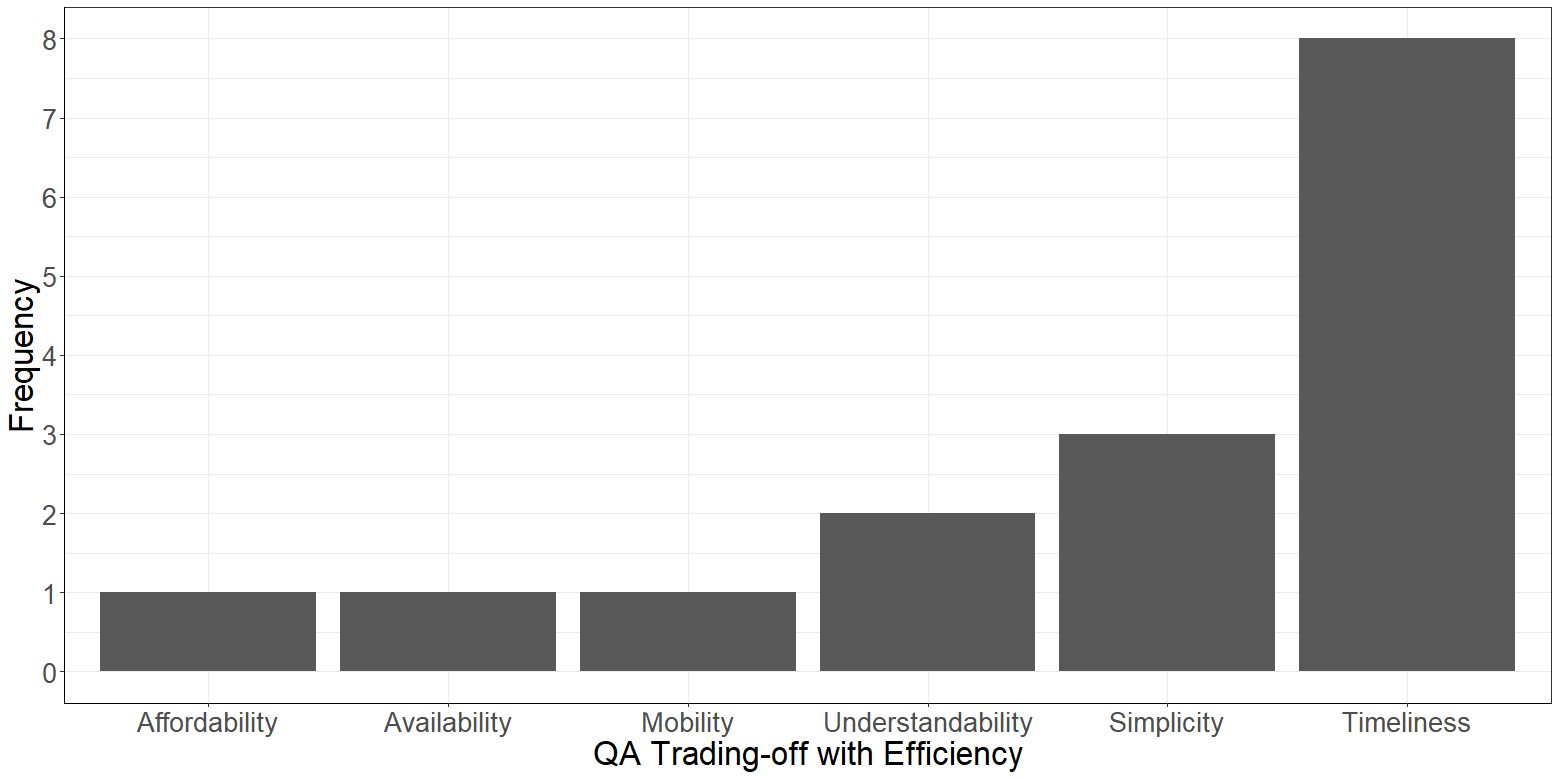
\includegraphics[width=250pt]{figures/trade_off_freq.png}
    \caption{QA Trade-off with Efficiency frequency distribution}
    \label{fig:trade_off_freq}
\end{figure}

\vspace{5mm}

It can be observed from figure \ref{fig:trade_off_freq} that the most common QA to trade-off with Efficiency is \textbf{Timeliness}.
This is to be expected as one can reason with common sense that when, f.e. speed is decreased to increase Efficiency, Timeliness will decrease.

Under Timeliness one could also understand the notion of \textit{Performance}, but considering that this is not an official
system's Quality Attribute, it can be explained as Timeliness.

- \textbf{Affordability} trades-off with Efficiency as improving Efficiency can require an increase in cost for the developer.
For example, the addition of subrobots to reduce the loss of traction by the weight of the payload.

- \textbf{Availability} trades-off with Efficiency as improving Efficiency can require the robot to reject stimuli when it predicts
that the stimuli will cost too much or waste energy \cite{kirtay2013humanoid_emotion}.

- \textbf{Mobility} trades-off with Efficiency as improving Efficiency can require the robot to limit stops, turns, directional changes and the degree 
to which the direction is changed as much as possible. This significantly reduces the Mobility of the robot.

- \textbf{Understandability} trades-off with Efficiency as improving Efficiency can require the robot to be more complicated in terms of hardware
and/or software. 
The added complexity; like an improved, more complex, algorithm which improves energy efficiency, can reduce the Understandability of the system.

- \textbf{Simplicity} trades-off with Efficiency as improving Efficiency can require the system to be expanded in a trivial manner, thus not
reducing the Understandability of the system but nonetheless making it more complex. Like adding the aforementioned subrobots to the system.

- \textbf{Timeliness} trades-off with Efficiency as improving Efficiency can require the robot to take the longer route instead of the shortest route
as the shortest route might contain more stops and turns, which is to be limited as much as possible.

\vspace{5mm}

Besides the fact that certain QA's need to be traded-off in order to improve energy efficiency, the extent to which this is required 
matters just as much, if not more.
For each system, the hit to the traded-off QA and the improvement of Efficiency will be significantly different.
Thus, an indication of expected percentages cannot be given.
However, with common sense it can be reasoned that a disproportional hit to the traded-off QA relative to the increase in Efficiency might not be worthwile.

Study \cite{kaitwanidvilai2020industrial_robot_cycle_time} for example states: "This method reduces energy consumption from 8155.20 to 7148.6 J, 
a decrease of 12.3\%.  On the other hand, the total moving time is increased by 71.8\% from 6.60 to 11.34 s". 
In case the system in question can suffer a 71.8\% reduction in Timeliness for a 12.3\% increase in Efficiency, it might be worthwile.
However, it can be considered a good example of a trade-off which might not be worthwile for most systems, let alone time-critical systems.

\vspace{5mm}

\noindent\fcolorbox{black}[HTML]{FFFFFF}{\parbox{0.47\textwidth}{%
\noindent \textbf{Main Findings.}
\begin{enumerate}[nolistsep]
\item The most common QA trade-off relative to Efficiency is \textbf{Timeliness}.
\item Some studies present QA trade-offs which are easily worthwile, like the reduction of Simplicity in favor of an increase in Efficiency.
\item Some QA trade-offs are not worthwhile for most robotic systems, like the reported 12.3\% increase in Efficiency for a 71.8\% decrease in Timeliness.
\end{enumerate}}}
 
\section{Discussion}
\label{sec:discussion}
This section will motivate the expansion of research into the energy impact of running the robotics software itself.
As described numerously in this literature study, this study aimed to give insights into the state-of-the-art of research
on the energy efficiency impact of software aspects in robotics software.
However, it became quickly apparant after the initial search that such studies were not numerous.
Out of the 683 potentially relevant studies, 17 primary studies were selected based on the application of the selection criteria, 
from which two studies would classify as a study into the energy efficiency impact of the robotics software itself.

Their publication dates are 2017 \cite{hou2017novel_cloud_evaluation_model} and 2019 \cite{rahman2019cloud_robot_offloading}, 
indicating the infancy of the field of study.

The importance of such research is significant, considering the high emmisions and use of energy in the automation sector, as explained
in section \ref{sec:intro}.
This literature study has mainly studied papers improving the energy efficiency of physical inefficiencies, 
be it the loss of traction (physical), the use of an FPGA\footnote{Field Programmable Gate Array} in combination with a neural network
to improve the acceleration on-board (hardware) or the improvement of an inefficient path finder (software).

One could thus say with confidence that, while there is still much to gain from that field, the impact of software itself is mostly left out
of the picture. 
As our society puts a growing effort towards a sustainable future, it warrants the expansion of research into this field of study.
The biggest improvement in energy efficiency is going to be achieved by combining all the aforementioned state-of-the-art methods for improving 
energy efficiency in section \ref{sec:results:rq2_state_of_the_art}, with software that is designed to be as energy efficient as possible.
This is already partly possible because of the contributions of \cite{hou2017novel_cloud_evaluation_model}, however the fact that this is the only paper
out of 17 primary studies, selected from 683 potentially relevant studies, which explicitly focuses on the identification of energy inefficient software, should warrant motivation for
the expansion of such research.
\section{Threats To Validity}\label{sec:threats}
\subsection{Internal Validity}
This threat has been mitigated as much as possible by defining the research protocol, as explained in section \ref{sec:study_design}, 
as rigorously as possible.
Iteratively defining it by discussing it after each iteration with my supervisor.

\subsection{External Validity}
The most severe potential external threat to the validity of this literature study is that the primary studies would not 
be representative of the state-of-the-art on energy efficiency in robotics software.

To avoid this to happen, the search strategy applied consisted of both automatic search and backward and forward snowballing 
\cite{wohlin2014snowballing}. Specifically, the presence of potential gaps left out by the automatic search was mitigated by 
the snowballing technique. 

This enlarged the set of relevant studies by considering each study selected in the automatic search, 
and focussing on those papers either citing or cited by it. 
Also, only peer-reviewed papers were considered and secondary and tertiary studies exlcuded.
This potential bias did not significantly impact this literature study, since the considered papers have undergone a rigorous
peer-review process, which is a well-established requirement for high quality publications. 

The inclusion and exclusion criteria were also rigorously and iteratively defined, again discussing it with my supervisor,
before the study design was put into action.

\subsection{Construct Validity}
This potential bias was mitigated by automatically searching the studies on any data source as indexed by \textbf{Google Scholar}.
The search string was also kept as general as possible, as explained before in section \ref{sec:study_design:search_selection}.

\subsection{Conclusion Validity}
Potential biases during the data extraction process were mitigated by rigorously and iteratively defining the data sheet with my superivsor.
By doing so, the alignment of the data extraction process with the research questions was guaranteed.
Furthermore, any potential threats to conclusion validity were mitigated, in general, by applying the best practices on systematic
literature reviews in each phase of this study, as stated in 
\cite{petersen2015guidelines_systematic, kitchenham2013systematic_review_guidelines, wohlin2012experimentation}.

This makes this literature study easy to be checked and replicated by other researchers.
\section{Conclusions}\label{sec:conclusions}
This literature study has given an insightful overview of the state-of-the-art in scientific literature on analyzing and improving 
energy efficiency in robotics software and identified trade-offs typically associated with such improvements.
Despite the already gained improvements in CO2 emmissions and energy consumption over the past years, as mentioned in section \ref{sec:intro}, 
Fysikopoulos et al. \cite{fysikopoulos2012automotive_energy_consumption} assert that 20\% to 40\% unnecessary use of energy may 
still be found in industrial firms.

The motivation for the expansion of research into the energy impact of robotic software \textit{itself} has been given in section \ref{sec:discussion}
and is a significant contribution of this literature study. 

\bibliographystyle{IEEEtran}
\bibliography{references}

\clearpage
\appendices

\section{Primary Studies}
\label{appendix:primary_studies}

\begin{table}[h]
    \centering
    \caption{Collection of primary studies.}
    \begin{tabular}{lp{5cm}p{9cm}c}
        \toprule
            {ID}
                {Publication Type} & 
                {Authors} & 
                {Title} &
                {Date} \\
        \midrule
            {1.}
                {conferencePaper} &
                {Mei, Yongguo; Lu, Yung-Hsiang; Lee, CS George; Hu, Y. Charlie} &
                {Energy-efficient mobile robot exploration} &
                {2006} \\
            \hline
            \\
            {2.}
                {journalArticle} &
                {Xie, Li; Henkel, Christian; Stol, Karl; Xu, Weiliang} &
                {Power-minimization and energy-reduction autonomous navigation of an omnidirectional Mecanum robot via the dynamic window approach local trajectory planning} &
                {2018} \\
            \hline
            \\
            {3.}
                {conferencePaper} &
                {Wigström, Oskar; Lennartson, Bengt} &
                {Sustainable production automation-energy optimization of robot cells} &
                {2013} \\
            \hline
            \\
            {4.}
                {conferencePaper} &
                {Cheng, Haoxuan; Sato, Shimpei; Nakahara, Hiroki} &
                {A Performance Per Power Efficient Object Detector on an FPGA for Robot Operating System (ROS)} &
                {2018} \\
            \hline
            \\
            {5.}
                {conferencePaper} &
                {Licea, Daniel Bonilla; McLernon, Des; Ghogho, Mounir; Zaidi, Syed Ali Raza} &
                {An energy saving robot mobility diversity algorithm for wireless communications} &
                {2013} \\
            \hline
            \\
            {6.}
                {conferencePaper} &
                {Kırtay, Murat; Oztop, Erhan} &
                {Emergent emotion via neural computational energy conservation on a humanoid robot} &
                {2013} \\
            \hline
            \\
            {7.}
                {journalArticle} &
                {Rahman, Akhlaqur; Jin, Jiong; Rahman, Ashfaqur; Cricenti, Antonio; Afrin, Mahbuba; Dong, Yu-ning} &
                {Energy-efficient optimal task offloading in cloud networked multi-robot systems} &
                {2019} \\ 
            \hline
            \\ 
            {8.}
                {journalArticle} &
                {Gürel, Sinan; Gultekin, Hakan; Akhlaghi, Vahid Eghbal} &
                {Energy conscious scheduling of a material handling robot in a manufacturing cell} &
                {2019} \\
            \hline
            \\
            {9.}
                {conferencePaper} &
                {Huh, Sungju; Hong, Seongsoo; Lee, Joonghyun} &
                {Energy-efficient distributed programming model for swarm robot} &
                {2013} \\    
            \hline
            \\
            {10.}
                {conferencePaper} &
                {Kim, Jeongwan; Dietz, J. Eric; Matson, Eric T.} &
                {Modeling of a multi-robot energy saving system to increase operating time of a firefighting robot} &
                {2016} \\
            \hline
            \\
            {11.}
                {journalArticle} &
                {Benkrid, Abdenour; Benallegue, Abdelaziz; Achour, Noura} &
                {Multi-robot Coordination for Energy-Efficient Exploration} &
                {2019} \\
            \hline
            \\
            {12.}
                {journalArticle} &
                {Kaitwanidvilai, Somyot; Chanarungruengkij, Veerasak; Konghuayrob, Poom} &
                {Remote Sensing to Minimize Energy Consumption of Six-axis Robot Arm Using Particle Swarm Optimization and Artificial Neural Network to Control Changes in Real Time} &
                {2020} \\
            \hline
            \\
            {13.}
                {conferencePaper} &
                {Barili, A.; Ceresa, M.; Parisi, C.} &
                {Energy-saving motion control for an autonomous mobile robot} &
                {1995} \\
            \hline
            \\
            {14.}
                {conferencePaper} &
                {Jia, Menglei; Zhou, GuangMing; Chen, ZongHai} &
                {An efficient strategy integrating grid and topological information for robot exploration} &
                {2004} \\
            \hline
            \\
            {15.}
                {journalArticle} &
                {Hou, Gang; Zhou, Kuanjiu; Qiu, Tie; Cao, Xun; Li, Mingchu; Wang, Jie} &
                {A novel green software evaluation model for cloud robotics} &
                {2017} \\
            \hline
            \\
            {16.}
                {conferencePaper} &
                {Mei, Yongguo; Lu, Yung-Hsiang; Hu, Y. Charlie; Lee, CS George} &
                {A case study of mobile robot's energy consumption and conservation techniques} &
                {2005} \\      
            \hline
            \\
            {17.}
                {conferencePaper} &
                {Patel, Sonali; Shukla, Anupam; Tiwari, Ritu} &
                {Efficient strategy for co-ordinated multirobot exploration} &
                {2012} \\
        \bottomrule
    \end{tabular}
    \label{table:primary_studies}
\end{table} \clearpage
\section{Data Sheet Part 1}
\label{appendix:data_sheet_1}

\begin{table}[h]
    \centering
    \caption{Data Sheet Part 1}
    \begin{tabular}{p{0.1cm}p{3cm}p{4cm}p{4cm}p{4cm}}
        \toprule
            {ID} &
                {Energy Metric}      & 
                {QA Trade-off}       & 
                {Application Domain} &
                {Identified Major Consumers}    \\
        \midrule
            {1.} &
                {Units of Energy} &
                {Performance Efficiency vs Energy Efficiency} &
                {Robot Exploration} &
                {Stops, turns, accelerating, decellerating, sensor distance waste, 
                inefficient algorithm for path finding} \\
            \hline
            \\
            {2.} &
                {Power: Watts (W)
                Energy: Joules (J)} &
                {Response vs Energy Efficiency} &
                {Robot Exploration} &
                {Big change in direction} \\
            \hline
            \\
            {3.} &
                {Joules (J)} &
                {Maintainability vs Energy Efficiency} &
                {Industrial Robot} &
                {Idle time} \\
            \hline
            \\
            {4.} &
                {FPS / W (Watts)} &
                {Maintainability vs Energy Efficiency} &
                {Service Robot} &
                {Inefficient use of robot hardware} \\
            \hline
            \\
            {5.} &
                {J / M (Joules / Meter)} &
                {Performance Efficiency vs Energy Efficiency} &
                {Wireless Robot Communication} &
                {Inefficiency of sending data over bad connection} \\
            \hline
            \\
            {6.} &
                {\textbf{NOT GIVEN}} &
                {Reliability vs Energy Efficiency} &
                {Service Robot} &
                {Processing of stimuli which costs too much energy} \\
            \hline
            \\
            {7.} &
                {Joules (J)} &
                {Performance Efficiency vs Energy Efficiency} &
                {Robot Exploration} &
                {Inefficient on-board computations instead of off-loading} \\
            \hline
            \\
            {8.} &
                {KiloJoules (KJ)} &
                {Performance Efficiency vs Energy Efficiency} &
                {Industrial Robot} &
                {Idle time} \\
            \hline
            \\
            {9.} &
                {\textbf{NOT GIVEN}} &
                {Maintainability vs Energy Efficiency} &
                {Wireless Robot Communication} &
                {Redudant data transmission} \\
            \hline
            \\
            {10.} &
                {Power: W / h (Watts)
                Energy: J / h (Joules)} &
                {Maintainability vs Energy Efficiency} &
                {Firefighting Robot} &
                {Loss of friction due to weight of payload} \\
            \hline
            \\
            {11.} &
                {\textbf{NOT GIVEN}} &
                {Maintainability vs Energy Efficiency} &
                {Robot Exploration} &
                {Redundancy / Inefficiency in overlap in paths} \\
            \hline
            \\
            {12.} &
                {Joules (J)} &
                {Performance Efficiency vs Energy Efficiency} &
                {Industrial Robot} &
                {Accelerating, Maintaining Speed, Decelerating, Idle time} \\
            \hline
            \\
            {13.} &
                {Power: W / h (Watts)
                Energy: KiloJoules (KJ)} &
                {Performance Efficiency vs Energy Efficiency} &
                {Robot Exploration} &
                {Obstacle avoidance without energy in mind} \\
            \hline
            \\
            {14.} &
                {\textbf{NOT GIVEN}} &
                {Performance Efficiency vs Energy Efficiency} &
                {Robot Exploration} &
                {Inefficient path planner} \\
            \hline
            \\
            {15.} &
                {NanoJoule (nJ)} &
                {\textbf{NOT GIVEN}} &
                {Energy Consumption Analysis} &
                {Poor quality software} \\
            \hline
            \\
            {16.} &
                {Power: Watts (W)} &
                {\textbf{NOT GIVEN}} &
                {Energy Consumption Analysis} &
                {Motion is the major consumer} \\
            \hline
            \\
            {17.} &
                {Units of Energy} &
                {Performance Efficiency vs Energy Efficiency} &
                {Robot Exploration} &
                {More than one robot moving to a target, 
                Robot assigned to target is not most efficient,
                Robots colliding on their way to targets} \\
        \bottomrule
    \end{tabular}
    \label{table:data_sheet_part_1}
\end{table} \clearpage
\section{Data Sheet Part 2}
\label{appendix:data_sheet_2}

\begin{table}[h]
    \centering
    \caption{Data Sheet Part 2}
    \begin{tabular}{p{0.1cm}p{5cm}p{3cm}p{2cm}p{2cm}p{4cm}p{5cm}}
        \toprule
            {ID} &
                {Identified Improving Software Aspect}    &
                {Major Contribution} &
                {Experiment}         &
                {Comparison}         &
                {Energy Model}       \\
        \midrule
            {1.} &
                {Improved algorithm, not wasting sensor distance, limit nr of stops etc, 
                target selection based on orientation instead of utility} &
                {The improved algorithm} &
                {Simulation} &
                {Yes} &
                {1 Unit of Distance = 1 Unit of Energy.
                Each stop = 0.5 Units of Energy.
                Each 45° degree turn = 0.4 Units of Energy,
                Each additional 45° of turn adds 0.2 units of Energy.} \\
            \hline
            \\
            {2.} &
                {Extended Dynamic Window Approach (DWA)} & 
                {Extended DWA with Energy Cost} &
                {Simulation} &
                {Yes} &
                {Mathematical Kinematics} \\
            \hline
            \\
            {3.} &
                {Scheduling algorithm reducing idle time} &
                {The scheduling algorithm} &
                {Simulation} &
                {Yes} &
                {Page 2 to 4} \\
            \hline
            \\
            {4.} &
                {Use of an FPGA} &
                {The complete system; using an FPGA in combination with a neural network} &
                {Real-world} &
                {Yes} &
                {Page 2} \\
            \hline
            \\
            {5.} &
                {Algorithm that would look for a better connection} &
                {Elaborate algorithm, finding best transmit location} &
                {Simulation} &
                {Yes} &
                {Page 2 to 4} \\
            \hline
            \\
            {6.} &
                {Trained neural network that would reject such stimuli} &
                {The actual trained neural network} &
                {Simulation} &
                {No} &
                {Page 3} \\
            \hline
            \\
            {7.} &
                {Off-loading to cloud or more available robot} &
                {An algorithm off-loading to more available robots or the cloud when more efficient} &
                {Simulation} &
                {Yes} &
                {Page 8 to 11 AND page 13} \\
            \hline
            \\
            {8.} &
                {Scheduling algorithm reducing idle time} &
                {The scheduling algorithm} &
                {Real-world} &
                {Yes} &
                {Page 3 to 7} \\
            \hline
            \\
            {9.} &
                {Reducing redundant data} &
                {Applying distributed systems paradigm MapReduce to reduce redundant data} &
                {Simulation} &
                {Yes} &
                {\textbf{NOT GIVEN}} \\
            \hline
            \\
            {10.} &
                {Adding subrobots carrying the weight} &
                {The complete system of subrobots, with the distributed systems algorithm to 
                facilitate communication} &
                {Simulation} &
                {Yes} &
                {\textbf{NOT GIVEN}} \\
            \hline
            \\
            {11.} &
                {Improved path finder} &
                {The improved path finder} &
                {Combination} &
                {Yes} &
                {page 3 to 4} \\
            \hline
            \\
            {12.} &
                {Balancing cycle time with major consumers} &
                {Algorithm balancing cycle time with major consumers} &
                {Simulation} &
                {Yes} &
                {page 3 to 4} \\
            \hline
            \\
            {13.} &
                {Trajectory planning with energy in mind} &
                {On-board trajectory planning with energy in mind} &
                {None} &
                {No} &
                {\textbf{NOT GIVEN}} \\
            \hline
            \\
            {14.} &
                {Improved path planner} &
                {Path planner with CostOverflow (CO) added, to get optimal time-energy paths} &
                {Combination} &
                {Yes} &
                {Page 3 to 4} \\
            \hline
            \\
            {15.} &
                {Ability to analyse energy consumption of software} &
                {A novel green evaluation method for software} &
                {Combination} &
                {Yes} &
                {\textbf{NOT GIVEN}} \\
            \hline
            \\
            {16.}  &
                {\textbf{NOT GIVEN}} &
                {A detailed study, identifying major consumers} &
                {Real-world} &
                {No} &
                {Page 2 to 4} \\
            \hline
            \\
            {17.}  &
                {An algorithm preventing given consumers} &
                {The entire system, including the algorithm mentioned} &
                {Simulation} &
                {Yes} &
                {Same as study 1} \\
        \bottomrule
    \end{tabular}
    \label{table:data_sheet_part_2}
\end{table}

\end{document}
